\section{Experiments}
\label{sec:exp}

\providecommand{\ci}[1]{\textnormal{\textcolor{gray}{\scriptsize$\pm$#1}}}



\begin{table}[t]
\centering
\caption{\textbf{Results across MolmoSpace tasks.} We evaluate all models on four manipulation skill categories---Pick, Pick \& Place, Open, and Close---and report mean success rate (\%) with standard error across three independent evaluation runs. \textbf{Bold} denotes the best and \underline{underline} the second-best per task. MolmoAct2-DROID achieves the highest overall average (37.7), outperforming the strongest prior baseline $\pi_{0.5}$-DROID (34.5) by +3.2 points, with particularly large gains on Pick (+7.3) and Pick \& Place (+13.1), where contact-rich, multi-stage reasoning is required. On Close, MolmoAct2-DROID also sets a new best at 70.8, while on Open it trails the leading methods, suggesting that articulated-object interaction remains a direction for further improvement. Standard errors remain comparable across methods ($\leq 3.2$), indicating that the observed gains are stable across runs rather than artifacts of evaluation variance.}
\label{tab:ms_results}
\begin{tabular}{lccccc}
% \toprule
\textbf{Models/Tasks} & \textbf{Pick} & \textbf{Pick \& Place} & \textbf{Open} & \textbf{Close} & \textbf{Average} \\
\midrule
% \multicolumn{6}{@{}l}{\textbf{\textit{Open weights only}}} \\
StereoVLA ~\citep{deng2025stereovla}           & 7.0\ci{2.3} & --   & -- & -- & 7.0 \\
LAP-VLA ~\citep{zha2026lap}            & 24.9\ci{2.7} & 6.6\ci{1.6}   & \underline{11.4}\ci{1.5} & 45.9\ci{2.9} & 22.2 \\
$\pi_{0}$-DROID ~\citep{black2410pi0}    & 16.2\ci{2.6} & 12.5\ci{2.0} & 11.0\ci{2.0} & 53.1\ci{3.2} & 23.2 \\
$\pi_{0.5}$-DROID ~\citep{intelligence2025pi05visionlanguageactionmodelopenworld}  & \underline{36.4}\ci{2.9} & \underline{13.6}\ci{2.2} & \textbf{22.7}\ci{2.6} & \underline{65.1}\ci{3.1} & \underline{34.5} \\
% \midrule
% \multicolumn{6}{@{}l}{\textbf{\textit{Molmo family: Open weights, Open data, Open code}}} \\
{\color{ai2pink}\molmoacttdroid}         & \textbf{43.7}\ci{3.1} & \textbf{26.7}\ci{2.8} & 9.5\ci{2.0} & \textbf{70.8}\ci{3.0} & \textbf{37.7} \\
% \bottomrule

\end{tabular}
\end{table}


\begin{table}[t]
\centering
\caption{\textbf{Evaluation on simulation held-out environments.} Simulation success rates are evaluated over 1000 episodes per task. For pick-and-place tasks, we report both oracle success (first number, which is the success conditions being fulfilled at any timestep) and success at end (second number, the success conditions being fulfilled at the final timestep). The delta between captures both unstable/unsuitable placement and the inability of policies to determine when a specified task is already completed, e.g. by repeatedly picking up an object which has already been placed correctly. We additionally report the half-width of the 95\% confidence interval bounds for each result. \textbf{Bold} denotes the best and \underline{underline} the second-best per task.}
\label{tab:sim_results}
\resizebox{\textwidth}{!}{
\begin{tabular}{@{}l@{\hspace{0.5em}}lc|ccc|ccc|c}
&\textbf{Models/Tasks} & \textbf{Pick MSProc} & \textbf{Pick Classic} & \textbf{Pick} & \textbf{Pick Rand.-Cam.} & \textbf{Pick\&Place} & \textbf{PnP Next-To} & \textbf{PnP Color} & \textbf{Avg.} \\
\toprule
% \multirow{5}{*}{\rotatebox[origin=c]{90}{\textit{Baselines}}}
&StereoVLA~\citep{deng2025stereovla} & 6.6\ci{2.6} & 4.3\ci{1.5} & 1.1\ci{1.0} & - & - & - & - & - \\
%&X-VLA~\citep{Zheng2025XVLAST} & ~7 & -- & -- & -- & -- & -- & -- \\
&X-VLA~\citep{zheng2025x} & 3.3\ci{1.0} & 0.5\ci{0.5} & 0.7\ci{0.5} & 0.8\ci{0.5} & 0.1\ci{0.2}/0.1\ci{0.2} & 1.9\ci{0.9}/1.0\ci{0.7} & 0.9\ci{0.6}/0.5\ci{0.5} & 1.2 \\
&LAP-VLA~\citep{zha2026lap} & \underline{19.4}\ci{2.4} & 2.4\ci{1.0} & 3.1\ci{1.1} & 2.7\ci{1.0} & 3.81\ci{1.5}/1.59\ci{1.0} & 6.48\ci{2.8}/3.41\ci{2.1} & 3.1\ci{1.1}/1.5\ci{0.8} & 4.8 \\
&$\pi_{0.5}$-DROID~\citep{intelligence2025pi05visionlanguageactionmodelopenworld}& 18.1\ci{2.4} & \underline{6.4}\ci{1.5} & \underline{7.0}\ci{1.6} & \underline{8.0}\ci{1.9} & \underline{11.7}\ci{2.1}/\underline{7.6}\ci{1.7} & \underline{8.2}\ci{2.2}/\underline{6.2}\ci{1.9} & \underline{10.4}\ci{1.9}/\underline{6.7}\ci{1.6} & \underline{10.0} \\
&{\color{ai2pink}\molmoacttdroid} & $\mathbf{35.6}$\ci{3.0} & $\mathbf{18.9}$\ci{2.6} & $\mathbf{20.5}$\ci{2.6} & $\mathbf{15.4}$\ci{2.4} & $\mathbf{15.8}$\ci{2.4}/$\mathbf{7.8}$\ci{1.8} & $\mathbf{20.9}$\ci{2.6}/$\mathbf{14.4}$\ci{2.3} & $\mathbf{17.2}$\ci{2.5}/$\mathbf{8.8}$\ci{2.0} & $\mathbf{20.6}$ \\
%&DreamZero\citep{ye2026dreamzero} & 52.1 & 6.x & -- & -- & -- & -- & -- \\
% \bottomrule
\end{tabular}
}
\end{table}
% \begin{figure}[t]
%     \centering
%     \includegraphics[width=\linewidth]{figures/Untitled Diagram.drawio (93).png}
%     \caption{Your caption here.}
%     \label{fi}

\begin{table}[t]
\centering
\caption{\textbf{Success rates (\%) across manipulation tasks.} Each cell reports the percentage of successful trajectories out of 15 trials. \textbf{Bold} denotes the best and \underline{underline} the second-best per task.}
\label{tab:task_success}
\resizebox{\textwidth}{!}{%
\begin{tabular}{lcccccc}
% \toprule
\textbf{Models/Tasks} & \textbf{Apple on plate} & \textbf{Pipette in tray} & \textbf{Red cube in tape roll} & \textbf{Knife in box} & \textbf{Objects in bowl} & \textbf{Average} \\
\midrule
$\pi_{0.5}$-DROID~\citep{intelligence2025pi05visionlanguageactionmodelopenworld}& 66.7                    & 33.3                    & \underline{53.3}        & 26.7                    & \underline{46.2} & 45.2 \\
MolmoBot~\citep{deshpande2026molmob0t}          & \underline{86.7}        & \underline{53.3}        & 33.3                    & \underline{40.0}        & 28.6             & \underline{48.4} \\
{\color{ai2pink}\molmoacttdroid}         & \textbf{100.0}          & \textbf{86.7}           & \textbf{93.3}           & \textbf{93.3}           & \textbf{62.0}    & \textbf{87.1} \\
% \bottomrule
\end{tabular}%
}
\end{table}

\begin{table}[h]
\centering
\caption{\textbf{Success rates (\%) across manipulation tasks on the SO-100 platform.} Each cell reports the mean score over 15 trials, where partial credit is awarded for sub-task completion (0.25 for reaching, 0.5 for pickup, 1.0 for successful placement). \textbf{Bold} denotes the best and \underline{underline} the second-best per task.}
\label{tab:so100_task_success}
\resizebox{\textwidth}{!}{%
\begin{tabular}{lcccccc}
% \toprule
\textbf{Models/Tasks} & \textbf{Fork on plate} & \textbf{Stack blocks} & \textbf{Tissues in basket} & \textbf{Pen on notebook} & \textbf{Block in box} & \textbf{Average} \\
\midrule
SmolVLA~\citep{shukor2025smolvlavisionlanguageactionmodelaffordable}        & 3.3                  & 5.0                  & 0.0                  & 3.3                  & 0.0                  & 2.3 \\
$\pi_{0}$-SO100/101~\citep{chen2025depi}            & \underline{30.0}     & \underline{6.7}      & \underline{20.0}     & \underline{80.0}     & \textbf{90.0}        & \underline{45.3} \\
{\color{ai2pink}\molmoacttso} & \textbf{70.0}        & \textbf{20.0}        & \textbf{73.3}        & \textbf{86.7}        & \underline{33.3}     & \textbf{56.7} \\
% \bottomrule
\end{tabular}%
}
\end{table}



\begin{figure}[t]
    \centering
    
\includegraphics[width=\linewidth]{figures/benchmark_0.pdf}
   
   
   \caption{\textbf{Performance comparison on the RoboEval benchmark.}
(A) Task-wise success rates (\%) across eight manipulation tasks for Diffusion Policy, GR00T N1.5, X-VLA, $\pi_{0.5}$-DROID, and MolmoAct. MolmoAct achieves the highest or near-highest success rates on most tasks, with particularly strong performance on long-horizon tasks such as \textit{Pack Box} and \textit{Rotate Valve}. $\pi_{0.5}$-DROID is the strongest baseline overall, while other methods exhibit lower and more variable performance across tasks.
(B) Radar plot of normalized performance across behavioral and outcome metrics, averaged over all tasks (outer edge indicates best performance per metric). MolmoAct consistently dominates across nearly all metrics, indicating improvements not only in task success but also in efficiency, stability, and trajectory quality. \textit{Abbreviations:} CT = completion time, TL = trajectory length, JPL = joint path length, CPL = Cartesian path length, CJ = Cartesian jerk, JJ = joint jerk, SC = self-collisions, SL = slip count.}


\label{fig:roboeval-results}
\end{figure}




\definecolor{norapink}{RGB}{252, 224, 224}
\definecolor{noralavender}{RGB}{226, 226, 250}
\begin{table}[h]
\centering
\small
\caption{\textbf{LIBERO benchmark success rates} across four task categories (Spatial, Object, Goal, and Long-horizon) along
with the average performance. \molmoactt achieves the highest overall average success rate of 97.2\%, outperforming
all strong baselines, with strong performance across all categories, particularly scoring 100\% on the LIBERO-Object tasks. Furthermore improvement could be seem going from \molmoactt to \molmothink. \textbf{Bold} denotes the best and \underline{underline} the second-best per task.}
\begin{tabular}{lccccc}
% \toprule
\textbf{Baseline} & \textbf{Spatial} & \textbf{Object} & \textbf{Goal} & \textbf{Long} & \textbf{Average} \\
\midrule
TraceVLA~\citep{zheng2024tracevla}           & 84.6\% & 85.2\%          & 75.1\% & 54.1\% & 74.8\% \\
OpenVLA~\citep{kim2024openvla}            & 84.7\% & 88.4\%          & 79.2\% & 53.7\% & 76.5\% \\
SpatialVLA~\citep{qu2025spatialvla}         & 88.2\% & 89.9\%          & 78.6\% & 55.5\% & 78.1\% \\
CoT-VLA~\citep{zhao2025cot}            & 87.5\% & 91.6\%          & 87.6\% & 69.0\% & 83.9\% \\
$\pi_0$~\citep{black2410pi0}            & 96.8\% & 98.8\%          & 95.8\% & 85.2\% & 94.2\% \\
ThinkAct~\citep{huang2025thinkact}           & 88.3\% & 91.4\%          & 87.1\% & 70.9\% & 84.4\% \\
MolmoAct-7B-D~\citep{lee2025molmoactactionreasoningmodels}      & 87.0\% & 95.4\%          & 87.6\% & 77.2\% & 86.6\% \\
GR00T N1.7~\citep{gr00tn1_2025}         & 97.7\% & 97.5\%          & \underline{98.5\%} & \underline{94.4\%} & 97.0\% \\
$\pi_{0.5}$~\citep{intelligence2025pi05visionlanguageactionmodelopenworld}       & \underline{98.8\%} & 98.2\%          & 98.0\% & 92.4\% & 96.9\% \\
NORA-1.5 ~\citep{hung2025nora} & 97.3\% & 96.4\% & 94.5\% & 89.6\% & 94.5\% \\
{\color{ai2pink}\molmoactt}          & 97.8\% & \textbf{100.0\%} & 97.8\% & 93.2\% & \underline{97.2\%} \\
{\color{ai2pink}\molmothink}   & \textbf{98.8\%} & \underline{99.8\%} & \textbf{98.5\%} & \textbf{95.4\%} & \textbf{98.1\%} \\
% \bottomrule
\end{tabular}
\label{tab:baseline-comparison}
\end{table}




\begin{figure}[t]
    \centering
    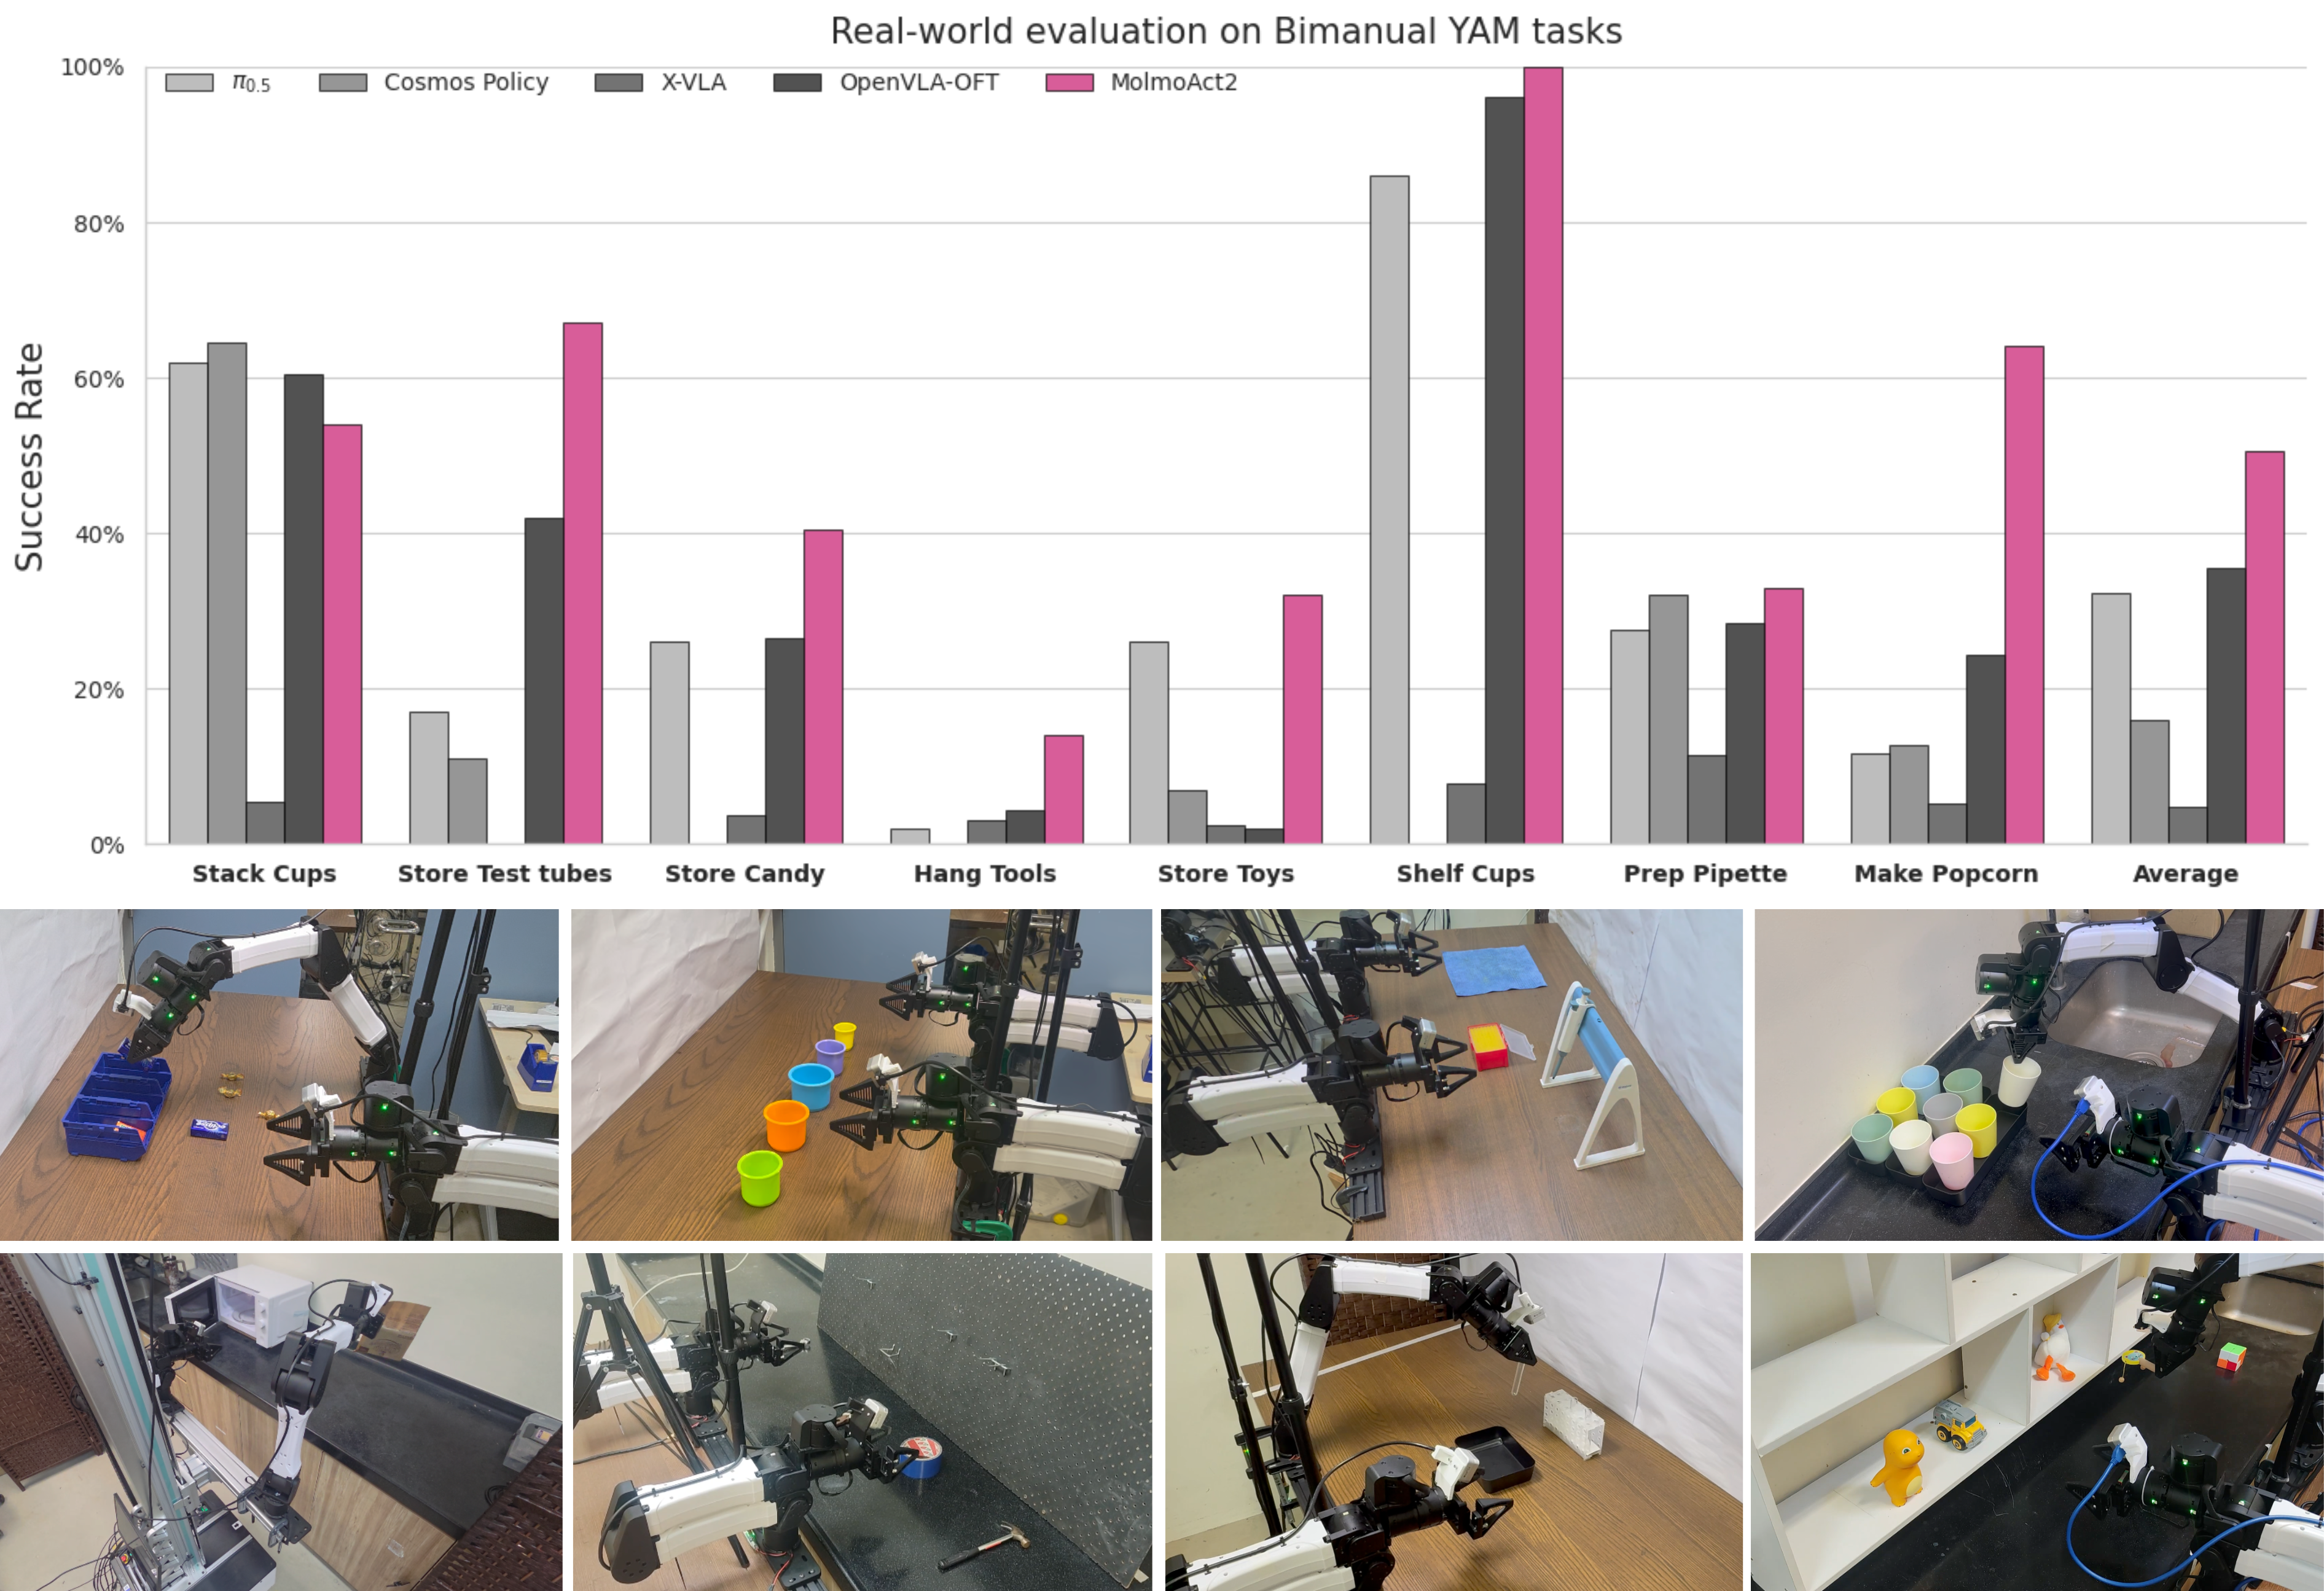
\includegraphics[width=\linewidth]{figures/MAF5.png}
    \caption{\textbf{Overview of efficient fine-tuning of \molmoactt.} 
We conduct a comprehensive evaluation across 8 real-world tasks outside of a 
laboratory setting, ranging from preparing a pipette for a chemist to placing 
toys back onto a shelf. \molmoactt, fine-tuned on the collected evaluation data, 
outperforms 4 strong baselines by a large margin of 15\% over the runner-up model.}
    \label{yamreal}
\end{figure}




Our experimental evaluation comprises one of the most extensive suites of studies of \molmoactt, benchmarked against a diverse set of strong generalist baseline models. Specifically, we assess \molmoactt across three main categories of evaluation: (i) we examine how \molmoer performs relative to generalist VLM models used as training backbones for VLAs, and quantify the performance gains attributable to a stronger backbone; (ii) we evaluate the out-of-the-box deployment capabilities of \molmoactt across a variety of embodiments; and (iii) we investigate the ease and efficiency with which \molmoactt can be adapted to novel tasks and unseen embodiments via fine-tuning. 

\noindent Hence, we evaluate \molmoactt across a comprehensive range of scenarios in both simulation and the real world, addressing the following research questions:

\begin{enumerate}
    \item \textbf{How well does \molmoer perform on established industry benchmarks for embodied reasoning in VLMs?} We address this question by benchmarking \molmoer against strong open-source and proprietary VLMs across 13 established embodied reasoning benchmarks.

    % \item \textbf{Does a stronger embodied reasoning VLM backbone improve action prediction?} We investigate this by evaluating \molmoactt on the LIBERO Long \citep{liu2023libero}, comparing performance when trained with the \molmot backbone against the \molmoer backbone.

    % \item \textbf{How effective is \molmoactfast compared to the closed-source FAST tokenizer for action prediction?} We investigate this by evaluating \molmoactt on the LIBERO simulation suite \citep{liu2023libero}, training with \molmoactfast and the FAST tokenizer \citep{pertsch2025fast} respectively.

    \item \textbf{How well does \molmoactt perform out-of-the-box?} We investigate this by evaluating \molmoactt on three benchmarks: two simulation benchmarks, MolmoBot~\citep{deshpande2026molmob0t} and MolmoSpaces~\citep{kim2026molmospaces}, and a series of real-world zero-shot evaluations across two embodiments (DROID and SO-100/101 setups) against strong baselines pretrained or fine-tuned on the DROID~\citep{khazatsky2024droid} and large-scale SO-100/101 datasets.

    % \item \textbf{How well does \molmoactt perform zero-shot in the SO-100/101 setup?}
    % We investigate this question by evaluating \molmoactt on a real-world benchmark designed to assess its zero-shot capabilities, comparing it against SmolVLA, which is also pretrained at scale on SO-100/101 data.

    \item \textbf{How effectively can \molmoactt be fine-tuned for new tasks and embodiments?} We study this by fine-tuning \molmoactt on custom datasets collected across three benchmarks: two simulation benchmarks, RoboEval \citep{wang2025roboeval} and LIBERO \citep{liu2023libero}, and one large-scale real-world evaluation suite consisting of in-the-wild bimanual YAM tasks.

    \item \textbf{Do adaptive depth-perception tokens improve the performance of \molmothink?}
    We investigate this question by comparing \molmoactt against \molmothink on LIBERO~\citep{liu2023libero}, MolmoSpace~\citep{kim2026molmospaces}, and the MolmoBot Benchmark~\citep{deshpande2026molmob0t}.

   \item \textbf{How robust is \molmoactt under out-of-distribution perturbations?} To investigate this, we fine-tune \molmoacttpos checkpoint on 4 tasks from the real-world Bimanual YAM benchmark and evaluate each task under 4 distinct out-of-distribution variants.

    \item \textbf{What is the quality of \molmoactt's trajectory rollouts beyond raw success rate?}
    For real-world deployment, trajectory quality matters beyond task success (e.g., stability, smoothness). We therefore evaluate \molmoactt against strong generalist baselines on RoboEval~\citep{wang2025roboeval} to assess the quality of the trajectories it generates while solving the tasks.

    \item \textbf{Which components contributed the largest performance gains to \molmoactt?}
    We investigate this question through systematic component-level ablations on the \molmoactt architecture and training configurations to understand how each of our novel improvements contributes to the model's performance, and we verify our findings on LIBERO~\citep{liu2023libero} for reproducibility.

    \item \textbf{How fast is \molmoactt at inference?}
    We measure end-to-end inference latency and control rate for \molmoactt and \molmothink on LIBERO~\citep{liu2023libero}, and evaluate the impact of our caching and CUDA Graph optimizations.

 

  
\end{enumerate}





\subsection{\molmoer evaluation}
\label{sec:exp-er}

\paragraph{Evaluation setup.} We evaluate \molmoer on 13 established vision-language benchmarks that are widely used to measure the embodied reasoning capabilities of VLMs: Point-Bench~\citep{cheng2025pointarena}, RefSpatial~\citep{zhou2025roborefer}, RoboSpatial-Point~\citep{song2025robospatial}, Where2Place~\citep{yuan2024robopoint}, BLINK~\citep{fu2024blink}, CV-Bench~\citep{tong2024cambrian}, ERQA~\citep{team2025gemini}, EmbSpatial~\citep{du2024embspatial}, MindCube~\citep{luopyspatial}, SAT~\citep{ray2025satdynamicspatialaptitude}, OpenEQA~\citep{majumdar2024openeqa}, and VSI-Bench~\citep{yang2025thinking}. Together, these benchmarks span visual question answering, 2D pointing, multi-image reasoning, ego–exo understanding, and video-based spatial reasoning. 

\paragraph{Baselines.}
We compare \molmoer against a diverse set of proprietary VLMs, reasoning-oriented VLMs, and open-weight VLMs, including the Gemini family~\citep{team2024gemini,comanici2025gemini}, the GPT-5 family~\citep{singh2025openai}, LLaVA-OneVision~\citep{li2024llava}, the Qwen3-VL family~\citep{bai2025qwen3}, and InternVLA~\citep{wang2025internvl3}. We additionally compare against \molmot~\citep{clark2026molmo2openweightsdata}, the base model from which \molmoer is trained.

\paragraph{Results.} \molmoer outperforms all baseline VLMs on 9 of the 13 benchmarks and achieves the highest overall average score of 63.8\%, exceeding the runner-up, Gemini-ER 1.5 Thinking, by 2.5 points. Notably, \molmoer improves over its base model \molmot by 17\%, demonstrating the substantial gains in embodied reasoning capability conferred by our approach.

\subsection{Out-of-the-box deployment}
\label{sec:exp-outbox}

\textbf{Evaluation setup and baselines.} To verify the out-of-the-box deployment capability of \molmoactt, we evaluate it in both simulation and real-world settings. In simulation, we evaluate the \molmoacttdroid checkpoint on two benchmarks: MolmoSpaces~\citep{kim2026molmospaces} and MolmoBot~\citep{deshpande2026molmob0t}. Both target single-cycle pick-and-place tasks across diverse objects and environments, with MolmoBot featuring more challenging objects and scenarios. Each benchmark replicates the original DROID~\citep{khazatsky2024droid} setup, enabling zero-shot evaluation of any policy pretrained or fine-tuned on the DROID dataset. On MolmoSpaces, we compare \molmoacttdroid against LAP-VLA~\citep{zha2026lap}, StereoVLA~\citep{deng2025stereovla}, $\pi_{0}$-DROID~\citep{black2410pi0}, and $\pi_{0.5}$-DROID~\citep{intelligence2025pi05visionlanguageactionmodelopenworld}; on MolmoBot, we compare against LAP-VLA, $\pi_{0.5}$-DROID~\citep{intelligence2025pi05visionlanguageactionmodelopenworld}, and X-VLA~\citep{zheng2025x}. All simulation evaluations strictly follow the protocols, trial counts, and procedures of the respective original papers. Further details are provided in the Appendix.

In the real world, we test \molmoacttdroid and \molmoacttso on their respective pretrained embodiment setups under challenging out-of-distribution conditions: camera poses are randomly initialized without conforming to any dataset visual distribution, using two cameras (wrist and a single allocentric view); all objects are unseen during training; and the environments themselves are out-of-distribution relative to the training data. For the DROID embodiment, we compare \molmoacttdroid against $\pi_{0.5}$-DROID~\citep{intelligence2025pi05visionlanguageactionmodelopenworld}, fine-tuned on the DROID dataset, and MolmoBot~\citep{deshpande2026molmob0t}, fine-tuned on the large-scale MolmoSpaces dataset. We evaluate on five tasks ranging from single- to multi-object pick-and-place: \texttt{apple\_on\_plate}, \texttt{pipette\_in\_tray}, \texttt{red\_cube\_in\_tape\_roll}, \texttt{knife\_in\_box}, and \texttt{objects\_in\_bowl}. For the SO-100/101 setup, we use the SO-100 robot, retaining the wrist camera and adding a third-person external camera with a randomly initialized position. We compare \molmoacttso against SmolVLA~\citep{shukor2025smolvlavisionlanguageactionmodelaffordable} and $\pi_{0}$-SO100/101, a variant of $\pi_{0}$ that we fine-tuned on \molmoacttsodata. Both baselines are pretrained or fine-tuned at scale on the SO-100/101 dataset. We evaluate five pick-and-place tasks with novel objects and randomly initialized camera poses. Every real-world policy is assessed over 15 trials, with partial credit awarded for near-successful executions. Further details are provided in the Appendix.

\textbf{Results.} \molmoacttdroid achieves strong zero-shot performance on all DROID-style setups, in both simulation and the real world. In simulation, \molmoacttdroid is the state-of-the-art VLA model across MolmoSpaces and MolmoBot, outperforming all baselines on both benchmarks. $\pi_{0.5}$-DROID is the runner-up on each, with \molmoactt achieving an absolute gain of $+10.6\%$ on MolmoBot and $+3.2\%$ on MolmoSpaces, averaged across tasks; trial counts in every case are sufficient for statistical significance. In real-world evaluation on the DROID setup, which is substantially more out-of-distribution given the random camera initialization and entirely novel scenes and objects relative to the DROID dataset~\citep{khazatsky2024droid}, \molmoactt again attains the highest performance, reaching $87.1\%$ and surpassing the runner-up MolmoBot by $38.7\%$. On the second zero-shot embodiment, SO-100/101, \molmoacttso reaches $56.7\%$, an $11.4\%$ gain over our open implementation of $\pi_{0}$ on SO-100/101, demonstrating affordable deployment on low-cost robots such as the SO-100/101.

\subsection{Effective fine-tuning}
\label{sec:exp-ft}

\textbf{Evaluation setups and baselines.} For rapid real-world deployment on novel tasks and embodiments, VLAs must adapt from only a handful of demonstrations. To assess \molmoact's capacity for such efficient adaptation, we benchmark it against several strong VLA baselines on downstream tasks, domains, and embodiments unseen during training. In all fine-tuning experiments, we initialize from the \molmoacttpos checkpoint and fine-tune on the benchmark-specific training data.

In simulation, we evaluate on two benchmarks. RoboEval~\citep{wang2025roboeval} comprises a bimanual Franka Emika Panda setup with human-expert demonstrations across 8 tasks requiring bimanual coordination. LIBERO~\citep{liu2023libero}, following prior work~\citep{kim2024openvla}, consists of four task suites—LIBERO-Spatial, LIBERO-Object, LIBERO-Goal, and LIBERO-Long—each containing 500 demonstrations across 10 tasks. We fully fine-tune \molmoactt and compare it against state-of-the-art VLAs trained under similar protocols, including TraceVLA~\citep{zheng2024tracevla}, OpenVLA~\citep{kim2024openvla}, SpatialVLA~\citep{qu2025spatialvla}, CoT-VLA~\citep{zhao2025cot}, $\pi_{0}$~\citep{black2410pi0}, ThinkAct~\citep{huang2025thinkact}, MolmoAct~\citep{lee2025molmoactactionreasoningmodels}, GR00T-N1~\citep{gr00tn1_2025}, $\pi_{0.5}$~\citep{intelligence2025pi05visionlanguageactionmodelopenworld}, and NORA-1.5~\citep{hung2025nora}.

For real-world evaluation, we conduct a large-scale, systematic study on both a bimanual YAM setup and a mobile bimanual YAM setup, covering 8 tasks that span static laboratory settings, in-the-wild environments (kitchen, study room, pantry, and wet labs), and mobile manipulation. The tasks—\texttt{stack\_cups}, \texttt{store\_test\_tubes}, \texttt{store\_candy}, \texttt{hang\_tools}, \texttt{store\_toys}, \texttt{shelf\_cups}, \texttt{prepare\_pipette}, and \texttt{make\_popcorn}—are each evaluated over 50 trials, with three spatial variants per task used for data collection. We fine-tune from the \molmoacttpos checkpoint for every task and compare against four strong VLA and world-model baselines: Cosmos Policy~\citep{kim2026cosmos}, X-VLA~\citep{zheng2025x}, OpenVLA-OFT~\citep{kim2025fine}, and $\pi_{0.5}$-DROID~\citep{intelligence2025pi05visionlanguageactionmodelopenworld}.

\textbf{Results.} On LIBERO, \molmoactt achieves an average success rate of 97.2\%, the highest among all compared methods—reaching 100\% on LIBERO-Object and improving over our previous MolmoAct-7B-D by 10.6\%. This trend is reinforced on RoboEval, where \molmoactt attains a 44.3\% success rate, surpassing the second-best model, $\pi_{0.5}$~\citep{intelligence2025pi05visionlanguageactionmodelopenworld}, by 3.8\%. In the real-world evaluation, \molmoactt outperforms all baselines on 7 of 8 deployment tasks, achieving an average success rate of 50.1\%—15\% above the runner-up, OpenVLA-OFT. Hence, \molmoactt demonstrate its effectiveness for rapid adaptation to new tasks, domains, and embodiments.

\subsection{Performance of \molmothink}
\label{depth}
To isolate the contribution of \molmothink, we fine-tuned it with the adaptive-depth training pipeline and compared it against \molmoactt, fine-tuned from \molmoacttpos under the standard recipe on LIBERO. \molmothink improves over \molmoactt on three of the four task suites and matches it on the fourth, where the baseline is already saturated at 100\%. Crucially, the largest gain (+2.2\%) appears on the most challenging suite, where the baseline leaves the most headroom (93.2\%), while gains on the easier suites are correspondingly smaller as performance approaches ceiling. Averaged across all suites and 2{,}000 rollouts, \molmothink achieves 98.1\% versus 97.2\%, a +0.9\% improvement that is consistent in sign and concentrated where the task is hardest which indicates that the adaptive-depth pipeline yields a real, non-incidental gain rather than noise around saturation.

\begin{table}[h]
\centering
\caption{\textbf{Robustness of \molmoactt{} under environmental perturbations.} 
We evaluate \molmoactt{} against four baselines on out-of-distribution scenarios 
spanning spatial variation, lighting, language rephrasing, and visual distractors. 
\molmoactt{} is the most robust, achieving an average success rate of 
\textbf{50.69\%} across all perturbation types—a \textbf{10.80\%} absolute 
improvement over the next-best model. Values report average success rates (\%); 
\textbf{bold} = best, \underline{underline} = second-best.}
\label{tab:perturbation_averages}
\begin{tabular}{lccccc}
\toprule
\textbf{Model} & \textbf{Spatial Var.} & \textbf{Lighting} & \textbf{Language} & \textbf{Distractor} & \textbf{Overall} \\
\midrule
$\pi_{0.5}$~\citep{intelligence2025pi05visionlanguageactionmodelopenworld}      & \underline{15.00}  & 33.70              & 26.15              & 33.20              & 27.01 \\
Cosmos Policy~\citep{kim2026cosmos}    & 8.75               & 17.50              & 5.00               & 13.75              & 11.25 \\
X-VLA~\citep{wen2025dexvla}     & 3.75               & 8.30               & 9.95               & 3.75               & 6.44 \\
OpenVLA-OFT~\citep{kim2025fine}   & 13.75              & \underline{46.25}  & \underline{51.25}  & \underline{48.30}  & \underline{39.89} \\
{\color{ai2pink}\molmothink}  & \textbf{26.25}     & \textbf{62.05}     & \textbf{60.35}     & \textbf{54.10}     & \textbf{50.69} \\
\bottomrule
\end{tabular}
\end{table}
\subsection{Robustness of \molmoactt to out-of-distribution shifts}
\textbf{Evaluation setup and baselines.} To investigate how robustly \molmoactt transfers after parameter-efficient fine-tuning on a new dataset, we select 4 of the 8 real-world bimanual tasks (\texttt{stack\_cups}, \texttt{store\_test\_tubes}, \texttt{store\_candy}, and \texttt{prepare\_pipette}) and fine-tune a separate checkpoint for each on top of \molmoacttpos. At test time, we evaluate each checkpoint under four out-of-distribution variants: \emph{spatial}, in which we place the target objects at locations outside the training distribution; \emph{lighting}, in which we alter the illumination of the scene; \emph{language variants}, in which we rephrase the language instruction in three different ways; and \emph{distractors}, in which we add unseen distractor objects while keeping the original in-distribution spatial layout. We compare \molmoactt to strong baselines such as $\pi_{0.5}$~\citep{intelligence2025pi05visionlanguageactionmodelopenworld}, Cosmos Policy~\citep{kim2026cosmos}, X-VLA~\citep{wen2025dexvla}, and OpenVLA-OFT~\citep{kim2025fine} .For each task each set, we will evaluate 20 trials, 5 trials for each perturbation. 

\textbf{Results.} Based on the evaluation, we find that \molmoactt is substantially more robust to perturbations than all other evaluated models, achieving a 50.7\% average success rate across all perturbation types, with a margin of $\sim$10.8\% over the second-best model, OpenVLA-OFT. While \molmoactt leads on every perturbation category, its advantage is narrowest on Distractor (a 5.8\% margin over OpenVLA-OFT), and it attains its lowest absolute score on Spatial Variance (26.25\%), indicating room for improvement on fine-grained spatial generalization.

\subsection{Quality of \molmoactt trajectories for real-world deployment}

While task success is a necessary measure of performance, it is insufficient for assessing readiness for real-world deployment. In practical settings, trajectory quality directly impacts efficiency, stability, and safety. We therefore evaluate \molmoactt fine-tuned on RoboEval for beyond success rates using a suite of behavioral and outcome metrics from RoboEval \citep{wang2025roboeval}, summarized in Fig.~\ref{fig:roboeval-results}B. Across tasks, \molmoactt demonstrates consistent improvements in efficiency-related metrics. For example, on \textit{Stack Two Blocks}, \molmoactt reduces completion time from $5.87$s ($\pi_{0.5}$) and $7.27$s (Diffusion) to $4.70$s, while also reducing joint path length from $2.16$ to $1.04$ (approximately $2\times$ shorter). Similar trends hold on longer-horizon tasks such as \textit{Rotate Valve}, where \molmoactt achieves the lowest completion time ($8.51$s vs.\ $9.69$s for $\pi_{0.5}$), along with reduced trajectory length.

In addition to efficiency, \molmoactt exhibits strong performance on stability-related metrics. As shown in Fig.~\ref{fig:roboeval-results}B, \molmoactt consistently operates near the best normalized value across both Cartesian and joint-space measures, indicating smoother and more stable trajectories compared to baselines. In contrast, other methods exhibit greater variability across these metrics, suggesting less consistent control behavior. Together, these results show that \molmoactt not only improves task success, but also produces shorter, more stable, and more efficient trajectories, which are critical properties for real-world deployment.

\subsection{Systematic analysis}
\label{sec:exp-systematic}

We ablate the main design choices in \molmoactt on \libero to isolate where the
performance gains come from. Unless otherwise noted, all variants use the same
data, image augmentation, action normalization, action horizon, and evaluation
protocol as the corresponding \libero fine-tuning run. For the full-suite
ablations, each row is evaluated on Spatial, Object, Goal, and Long, and the
average is computed across the four suites.

\paragraph{Embodied-reasoning backbone.}
We first test whether the \molmoer backbone improves action learning even before
the continuous action expert is introduced. We directly fine-tune \molmot and
\molmoer with the same discrete-action architecture on the single \libero Long
task suite, using action tokens produced by \molmoactfast and no continuous action expert. Both
models are trained for 60{,}000 steps with the same configuration. As shown in
\autoref{tab:ablation-er-backbone}, replacing \molmot with \molmoer improves
success from 77.6\% to 83.6\%, a 6.0-point gain. This confirms that the
embodied-reasoning specialization is not only useful for VLM benchmarks, but
also transfers directly into action-token prediction.

\begin{table}[h]
\centering
\caption{\textbf{Backbone ablation on \libero Long.} Both variants are trained
directly from the VLM checkpoint with only discrete action prediction using
\molmoactfast. The final row is marked in pink, which is what we initialize with
for \molmoacttpre.}
\begin{tabular}{lcc}
\textbf{Backbone} & \textbf{Action objective} & \textbf{Long} \\
\midrule
\molmot~\citep{clark2026molmo2openweightsdata} & Discrete & 77.6\% \\
{\color{ai2pink}\molmoer} & Discrete & \textbf{83.6\%} \\
\end{tabular}
\label{tab:ablation-er-backbone}
\end{table}

\paragraph{VLM-to-expert conditioning.}
We next ablate how the continuous action expert receives context from the VLM.
All variants start from \molmoacttpre, attach an action expert directly, and
use the same \libero training configuration. We compare hidden-state
conditioning, standard per-layer KV conditioning, and a per-head
per-layer KV conditioning variant. In the standard design, the VLM key and value heads at
each token are flattened before learned projections map them into the action
expert cross-attention space. In the per-head variant, the VLM keys and values remain
separated by head, and each head is projected into the corresponding
action-expert head. This preserves the head structure, but requires the number
of VLM KV heads to match the number of action-expert KV heads; we use 8 for
both in all settings. The standard per-layer KV conditioning is strongest on
average, reaching 95.9\%, compared with 94.8\% for the per-head variant and
94.0\% for hidden-state conditioning
(\autoref{tab:ablation-connection-source}).
Hidden-state conditioning is competitive on Spatial, but it drops more on
Object, Goal, and Long. This supports the architectural choice in
Sec.~\ref{sec:posttraining-action-expert}, where the action expert consumes the
same attention state used by the VLM rather than a single residual-stream
representation.

\begin{table}[h]
\centering
\caption{\textbf{Ablation of the VLM-to-action-expert conditioning source on
\libero.} All variants are trained from \molmoacttpre with the same
configuration. \textbf{Bold} denotes the best result per column. The final row is marked in pink, which is what we use in all \molmoactt and \molmothink post-training and fine-tuning runs.}
\begin{tabular}{lccccc}
\textbf{Conditioning source} & \textbf{Spatial} & \textbf{Object} & \textbf{Goal} & \textbf{Long} & \textbf{Average} \\
\midrule
Hidden-state conditioning & \textbf{97.0\%} & 95.4\% & 96.6\% & 87.0\% & 94.0\% \\
Per-head per-layer KV conditioning & 95.8\% & 97.2\% & 96.6\% & 89.6\% & 94.8\% \\
\color{ai2pink}{Per-layer KV conditioning} & 96.2\% & \textbf{99.0\%} & \textbf{98.6\%} & \textbf{89.8\%} & \textbf{95.9\%} \\
\end{tabular}
\label{tab:ablation-connection-source}
\end{table}

\paragraph{Multiple flow samples.}
We then vary the number of flow samples \(K\) per action chunk while holding
per-layer KV conditioning and all other training settings fixed.
These runs also start from \molmoacttpre without a prior post-training stage.
\autoref{tab:ablation-flow-steps} shows that increasing \(K\) generally
improves average performance. \(K=1\) is the weakest overall at 94.15\%,
while \(K=8\) gives the best average at 95.90\%.
The effect is not monotonic on every suite, because Long benefits strongly from
two flow samples, but the aggregate trend favors denser supervision along the flow
trajectory.

\begin{table}[h]
\centering
\caption{\textbf{Ablation of the number of flow samples on \libero.} All rows
use per-layer KV conditioning and are trained from \molmoacttpre with the same
configuration. \textbf{Bold} denotes the best result per column. The final row is marked in pink, which is what we stick to in all of \molmoactt and \molmothink fine-tuning runs.}
\begin{tabular}{cccccc}
\textbf{\(K\)} & \textbf{Spatial} & \textbf{Object} & \textbf{Goal} & \textbf{Long} & \textbf{Average} \\
\midrule
1 & 95.0\% & 95.8\% & 98.2\% & 87.6\% & 94.15\% \\
2 & \textbf{96.6\%} & 96.0\% & 95.4\% & \textbf{92.2\%} & 95.05\% \\
4 & 96.2\% & 98.4\% & 97.0\% & 89.0\% & 95.15\% \\
\color{ai2pink}8 & 96.2\% & \textbf{99.0\%} & \textbf{98.6\%} & 89.8\% & \textbf{95.90\%} \\
\end{tabular}
\label{tab:ablation-flow-steps}
\end{table}

\paragraph{Fine-tuning design.}
\autoref{tab:ablation-training-design} compares the final \molmoactt fine-tuning recipe
against targeted alternatives along three axes: whether we co-train the
discrete autoregressive action loss, whether we apply knowledge insulation to
the flow-matching loss, and which parameters are updated. Removing discrete
action co-training yields a similar average but shifts performance across
suites, improving Long while reducing Spatial and Object. Adding knowledge
insulation is also close but slightly worse than the final recipe. LoRA remains
strong, especially on Spatial, but loses 2.8 points on Long relative to full
fine-tuning. Tuning only the action expert is the clearest failure mode,
dropping the average to 93.05\%. Overall, full-model adaptation with discrete
and continuous action co-training provides the best average outcome.

\begin{table}[h]
\centering
\caption{\textbf{Ablation of \molmoactt fine-tuning design choices on
\libero.} Component columns indicate whether each design choice is enabled:
\textcolor{forestgreen}{\cmark} denotes enabled and \textcolor{darkred}{\xmark}
denotes disabled. \textbf{Bold} denotes the best result per column. The final row is the \molmoacttlib recipe, where its training design is marked in pink, which is what we stick to in all of \molmoactt fine-tuning runs.}
\resizebox{0.88\linewidth}{!}{%
\begin{tabular}{@{}cclccccc@{}}
\textbf{\makecell{Discrete\\co-training}} & \textbf{\makecell{Knowledge\\insulation}} & \textbf{Training type} & \textbf{Spatial} & \textbf{Object} & \textbf{Goal} & \textbf{Long} & \textbf{Average} \\
\midrule
\textcolor{darkred}{\xmark} & \textcolor{darkred}{\xmark} & Full fine-tuning & 95.8\% & 98.6\% & \textbf{98.4\%} & \textbf{95.0\%} & 96.95\% \\
\textcolor{forestgreen}{\cmark} & \textcolor{forestgreen}{\cmark} & Full fine-tuning & 96.8\% & 99.4\% & 97.2\% & 94.8\% & 97.05\% \\
\textcolor{forestgreen}{\cmark} & \textcolor{darkred}{\xmark} & LoRA & \textbf{98.0\%} & 99.4\% & 97.2\% & 90.4\% & 96.25\% \\
\textcolor{darkred}{\xmark} & \textcolor{darkred}{\xmark} & Action expert only & 91.6\% & 97.6\% & 93.8\% & 89.2\% & 93.05\% \\
\textcolor{ai2pink}{\cmark} & \textcolor{ai2pink}{\xmark} & {\color{ai2pink}Full fine-tuning} & 97.8\% & \textbf{100.0\%} & 97.8\% & 93.2\% & \textbf{97.20\%} \\
\end{tabular}%
}
\label{tab:ablation-training-design}
\end{table}

\paragraph{Depth-aware fine-tuning.}
Finally, we ablate the \molmothink depth fine-tuning recipe. The baseline
uses both 10\% depth-token noise and the learned per-layer depth gate described
in Sec.~\ref{sec:think-training}, while uniformly mixing action-only and
depth-and-action examples. Removing the depth-token noise and per-layer depth
gate reduces the average from 98.10\% to 97.65\%, mostly through a 1.8-point
drop on Goal. Removing mixed training as well, so that training uses only
depth-and-action examples, reduces the average further to 97.50\%. These
results show that the depth pathway is most useful when it is regularized for
imperfect inference-time depth predictions and when the policy retains a strong
action-only path.

\begin{table}[h]
\centering
\caption{\textbf{Ablation of \molmothink depth fine-tuning choices on
\libero.} Mixed training denotes uniform sampling of action-only and
depth-and-action examples. \textcolor{forestgreen}{\cmark} denotes enabled and
\textcolor{darkred}{\xmark} denotes disabled. \textbf{Bold} denotes the best result per column. The final all-enabled row is the \molmothinklibero recipe, where its training design is marked in pink, which is what we stick to in all of \molmothink fine-tuning runs.}
\resizebox{0.7\linewidth}{!}{%
\begin{tabular}{@{}cccccccc@{}}
\textbf{\makecell{Mixed\\training}} & \textbf{\makecell{Noise\\injection}} & \textbf{\makecell{Depth\\gate}} & \textbf{Spatial} & \textbf{Object} & \textbf{Goal} & \textbf{Long} & \textbf{Average} \\
\midrule
\textcolor{darkred}{\xmark} & \textcolor{darkred}{\xmark} & \textcolor{darkred}{\xmark} & 97.6\% & 99.6\% & 96.6\% & \textbf{96.2\%} & 97.50\% \\
\textcolor{forestgreen}{\cmark} & \textcolor{darkred}{\xmark} & \textcolor{darkred}{\xmark} & \textbf{98.8\%} & \textbf{99.8\%} & 96.6\% & 95.4\% & 97.65\% \\
\textcolor{ai2pink}{\cmark} & \textcolor{ai2pink}{\cmark} & \textcolor{ai2pink}{\cmark} & \textbf{98.8\%} & \textbf{99.8\%} & \textbf{98.4\%} & 95.4\% & \textbf{98.10\%} \\
\end{tabular}%
}
\label{tab:ablation-depth-training}
\end{table}


\subsection{Inference speed}
\label{speed}
We measure end-to-end action-generation latency on LIBERO using a single H100 GPU and an action horizon of 10, and report the amortized control rate as action horizon divided by latency. We compare three inference paths: the original implementation, an optimized eager path using reusable-cache optimizations, and the same optimized path with CUDA Graph replay enabled.

\begin{figure}[t]
  \centering
  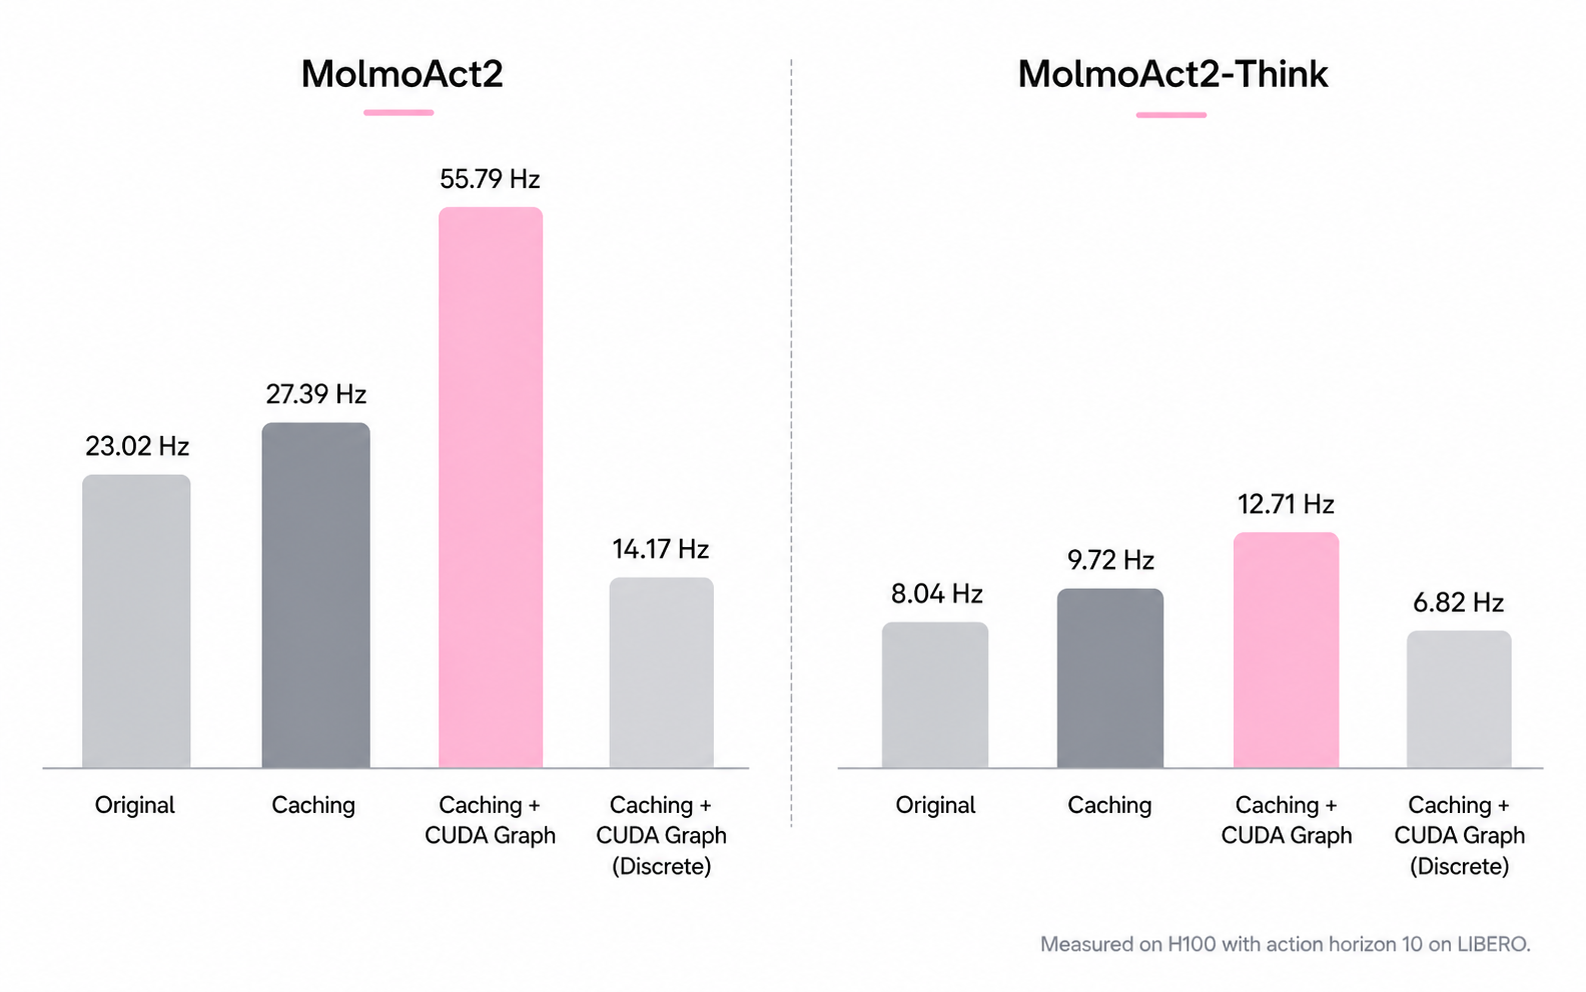
\includegraphics[width=0.78\linewidth]{figures/speedup.png}
  \caption{\textbf{Inference control rate after caching and CUDA Graph optimizations.} Control rate is action horizon divided by end-to-end action-generation latency; measurements use horizon 10 on LIBERO
with a single H100.}
  \label{fig:inference-speedup}
\end{figure}

As shown in \autoref{fig:inference-speedup}, caching alone improves \molmoactt from 23.02 Hz to 27.39 Hz and \molmothink from 8.04 Hz to 9.72 Hz. Enabling CUDA Graphs gives the larger gain: \molmoactt reaches 55.79 Hz, a 2.42\(\times\) speedup over the original path, while \molmothink reaches 12.71 Hz, a 1.58\(\times\) speedup. \molmoactt benefits substantially from CUDA Graph replay: its fixed-shape flow-matching steps form a regular, repeated computation pattern whose runtime is dominated by kernel launch overhead, which graph replay largely eliminates. \molmothink sees a smaller gain, since its adaptive-depth stage performs autoregressive decoding, whose sequential dependencies and variable-length execution are less amenable to graph capture.

\molmoactt also exposes a discrete action path, in which the VLM autoregressively decodes action tokens for the entire action chunk. We measured this path under the same optimized graph as above. \molmoactt runs at 14.17~Hz and \molmothink at 6.82~Hz i.e., \(3.94\times\) and \(1.86\times\) slower than the corresponding continuous path. This gap comes from the large VLM decoding overhead, while the action expert emits the entire chunk in a small fixed number of flow matching steps through a smaller cross-attention head, with the VLM cache reused across steps. We therefore use the continuous path as the default deployment option.
